\section{Linial's Algorithm}

A useful procedure is one that merges two linearly ordered sets without
discarding the information existing between elements of these two sets. In
\citet*{cardinal:2013} an implementation of such a procedure is defined. Their
implementation allows one to concentrate the computational complexity
in the preprocessing phase of their other algorithms. In this chapter
we detail another possible implementation of such a procedure that is due
to \citet*{linial:1984}. Unfortunately, in this implementation the
computational complexity cannot be split into a preprocessing phase and a query
phase. Nevertheless it is still interesting to understand the ideas behind it.

This procedure solves the problem of Merging under Partial Information
(\MUPI)\define{MUPI}. Note that \MUPI is a special case of \SUPI. The difference with
\SUPI is that together with the input poset \(\P\) we are given two chains \(\A
= (\chain{a_1}{a_m})\) and \(\B = (\chain{b_1}{b_n})\) such that \(\A \cup \B =
\P\), \ie \(\enum{\A,\B}\) is a chain cover of \(\P\), implying that \(\P\) is
of width \(2\). We give a formal definition of this problem,
\begin{problem}[Merging under Partial Information]
Given a poset \(\P\) and two disjoint chains \(\A\) and \(\B\) of \(\P\) such that \(\A \cup \B =
\P\), find a linear extension of \(\P\).
\end{problem}

\begin{figure}
\centering
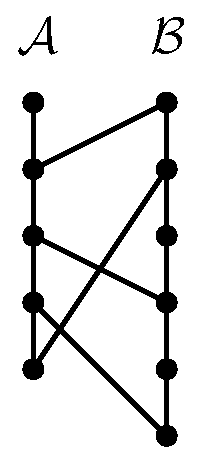
\includegraphics[height=0.2\textheight]{fig/supi/mupi}
\caption{A poset \(\P\) covered by two chains \(\A\) and \(\B\),
input of the \MUPI problem.}
\label{fig:supi:mupi}
\end{figure}

\citet*{linial:1984} first proves that the \onethirdtwothird conjecture holds
for width-\(2\) posets, \ie posets that can be covered by two chains. Since one
can always find a good query that when answered invalidates at
least one-third of the possible linear extensions of \(\P\), it is possible to design a
\BigO{\log e(\P)} algorithm that solves the \MUPI problem.
\begin{theorem}[\citet*{linial:1984}]
Given a poset \(\P\) covered by two chains \(\A\) and \(\B\), we can always find
a query \(x \ask{\le} y\) with \(x \in \A, y \in \B\) such that the probability
that \(x \le y\) lies in the interval \([\sfrac{1}{3}, \sfrac{2}{3}]\).
\end{theorem}

Moreover, in his proof, \citet*{linial:1984} shows that if we consider that \(
a_1\) and \(b_1\) are incomparable and \(\frac{e(\P(a_1 < b_1))}{e(\P)} <
\sfrac{1}{3}\) then there must exist an \(r\) for which either
\begin{displaymath}
\sfrac{1}{3} \le \frac{e(\P(a_1 < b_{r-1}))}{e(\P)} \le \sfrac{1}{2},
\end{displaymath}
or
\begin{displaymath}
\sfrac{1}{2} \le \frac{e(\P(a_1 < b_{r}))}{e(\P)} \le \sfrac{2}{3}.
\end{displaymath}

All of this is without loss of generality. If \(a_1\) and \(b_1\) are
comparable then either \(a_1\) or \(b_1\) is the unique minimal element of \(\P\).
Hence this minimal element can be removed. We can do so
until \(a_1\) and \(b_1\) are incomparable. If \(\frac{e(\P(a_1 < b_1))}{e(\P)} >
\sfrac{2}{3}\) we can simply revert the roles of \(\A\) and \(\B\) and if
\(\sfrac{1}{3} \le \frac{e(\P(a_1 < b_1))}{e(\P)} \le \sfrac{2}{3}\) then we
simply do not have to search any further. Also, one can build the same
proof using \(a_m\) and \(b_n\) instead of \(a_1\) and \(b_1\).

\citet*{linial:1984} proposes the following polynomial-time algorithm. We
compute the number of linear extensions of the width-\(2\) poset \(\P\) using
the determinant counting formula (which we explain later). We do so also for every query we could use to
retrieve more information on the total order \(\le\). We then use those counts
to find a pair \((x,y)\) that satisfies \(\sfrac{1}{3} \le \frac{e(\P(x \le
y))}{e(\P)} \le \sfrac{2}{3}\). Once this pair is
identified, we can effectively make the query and update poset \(\P\) with the
actual answer. We can then recurse on the newly obtained poset. Because of the
successive uses of good queries, the recursion depth, and thus the number of
queries made, is \BigO{\log e(\P)}.

The proof for the determinant counting formula \citet*{linial:1984} uses can be
found in \citet*{mohanty:1979}, we give hereunder the statement of this formula
in the context of Merging under Partial Information.
\begin{theorem}[\citet*{mohanty:1979}]
Let \(\P = \A \cup \B\), where \(\A = (\chain{a_1}{a_m})\) and \(\B =
(\chain{b_1}{b_n})\), and assume \(m \ge n\) without loss of generality. Define
the integers \(\alpha_1,\ldots,\alpha_m,\beta_1,\ldots,\beta_m\) as follows,
\(\beta_i = min\{t \st b_t > a_i\}, \alpha_j = max\{t \st b_t < a_j\}\) and
where the minimum and maximum of an empty set are taken to be \(n + 1\) and
\(0\) respectively. Let \(\binom{n}{k}_{+}\) be defined as
\begin{displaymath}
\binom{n}{k}_{+} =
\begin{dcases*}
0            & if  \(n < 0\)  or \(k < 0\)  or \(k > n\)\\
1            & if \(k = 0\)  or \(k = n\)\\
\binom{n}{k} & otherwise\\
\end{dcases*}.
\end{displaymath}
Then, the number of linear extensions of \(\P\) is given by
\begin{displaymath}
e(\P) =
\begin{vmatrix}
\binom{\beta_i - \alpha_j}{j - i - 1}_{+}
\end{vmatrix}_{1 \le i , j \le m},
\end{displaymath}
the determinant of a \(m \times m\) matrix.
\end{theorem}

\citet*{mohanty:1979} gives this formula in the context of counting lattice
paths. Let us explain. We want to count the number of paths that go from
\((0,0)\) to \((m,n)\) in a \((m+1) \times (n+1)\) grid. Such a path is a
sequence of \(m+n+1\) integer positions \(( (i_{0},j_{0}) , (i_{1},j_{1}) ,
\ldots , (i_{m+n},j_{m+n}) )\) such that \(i_{k} \ge i_{k-1}\), \(j_{k} \ge
j_{k-1}\) and \(i_{k} + j_{k} = i_{k-1} + j_{k-1} + 1\) for all \(1 \le k \le m
+ n\).  Obviously \((i_{0},j_{0}) = (0,0)\) and \((i_{m+n},j_{m+n}) = (m,n)\).
With these constraints alone we obtain a count of \(\binom{m+n}{n} =
\binom{m+n}{m} \) different paths\footnote{Note that if \(m = n\) and if we add
the condition that \(i_{k} \le j_{k} \Forall 1 \le k \le m + n\) then the path
count corresponds to the \(\nth{n}\) Catalan number \(C_n\).}.
\citet*{mohanty:1979} adds the constraint that \(\alpha_i \le j < \beta_i\) for
all path positions \((i,j)\) with \(i \neq 0\), where \(0 \le
\alpha_1 \le \ldots \le \alpha_m \le n + 1\), \(0 \le \beta_1 \le \ldots \le
\beta_m \le n + 1\) and \(\alpha_i < \beta_i \Forall 1 \le i \le m\) and finds
this determinant counting formula as an answer. The reason the cases \(i = 0\)
can be ignored is because the above constraints suffice to fix
the possible values that \(j\) can take when \(i = 0\).

This problem of counting paths is equivalent to counting the number of possible
outcomes of a merging algorithm on input \((\S_1,\S_2)\), \(\card{\S_1} = m,
\card{\S_2} = n\), provided we know the insertion position \(j\) of the
\(\nth{i}\) element of \(\S_1\) into \(\S_2\) is bounded by \(\alpha_i \le j <
\beta_i\).

We now make a few observations to show that Linial's algorithm runs in
polynomial time:
\begin{enumerate}
\item The values \(\beta_i - \alpha_j\) and \(j - i + 1\) are bounded
linearly in the size of the input. Hence, their size is bounded
logarithmically in the size of the input;
\item The size of the value of the binomial coefficient \(\binom{n}{k}\) is
bounded by a polynomial in \(k\) and \(n\);
\item Using Bareiss algorithm~\cite{bareiss:1968}, the computation of a
determinant can be done in polynomial time. Moreover, the size of all computed
values is bounded by some polynomial in the size of the matrix and in the starting
size of the values;
\item For each step there is a polynomial number of possible queries to look for;
\item There are \BigO{\log e(\P)} steps and \(\log e(\P)\) is \BigO{n \log n}.
\end{enumerate}

However, the algorithm \emph{as is} is not practical. The complexity added
by the computation of binomial coefficients matrices and determinants in
Linial's algorithm is at least quadratic. In the next section, we present an
original implementation of this algorithm that uses dynamic programming to
avoid the computation of binomial coefficients and determinants.
